\date{}
\title{}
\date{}
\begin{document}
\begin{frame}
    \titlepage
\end{frame}

\section{routing problem}

\usetikzlibrary{matrix}
\begin{frame}{routing tables}
\begin{tikzpicture}
\matrix[tight matrix,
    nodes={minimum height=.6cm},gT
    column 1/.style={nodes={text width=4.5cm,font=\small\tt}},
    column 2/.style={nodes={text width=2cm,font=\small\tt,alt=<4>{fill=red!10}}},
    column 3/.style={nodes={text width=1cm,font=\small\tt,alt=<3>{fill=red!10}}},
    row 1/.style={nodes={font=\small}},
    label={north:routing table},
    anchor=north west
] (route table v6) {
IP addresses \& gateway \& iface \\
2001:0db8:40:f000:;/44 \& --- \& int1 \\
2001:0db8:40:e000::/44 \& 2001:0db8:40:f000::2 \& int1 \\
2001:0db8:40:d000::/44 \& --- \& int3 \\
3fff:1000:19::/48 \& --- \& ext1 \\
\ldots \& \ldots \& \ldots \\
\normalfont default \& fe80::17 \& ext2 \\
};
\matrix[tight matrix,
    nodes={minimum height=.6cm},gT
    column 1/.style={nodes={text width=4.5cm,font=\small\tt}},
    column 2/.style={nodes={text width=2cm,font=\small\tt,alt=<4>{fill=red!10}}},
    column 3/.style={nodes={text width=1cm,font=\small\tt,alt=<3>{fill=red!10}}},
    row 1/.style={nodes={font=\small}},
    label={north:routing table},
    anchor=north west
] (route table v4) at (route table v6.south west) {
IP addresses \& gateway \& iface \\
192.0.2.0/25 \& --- \& int1 \\
192.0.2.128/26 \& 192.0.2.1 \& int1 \\
192.0.2.192/26 \& 192.0.2.2 \& int1 \\
198.51.100.0/25 \& 192.0.2.1 \& int1 \\
198.51.100.128/25 \& --- \& int2 \\
\ldots \& \ldots \& \ldots \\
\normalfont default \& 203.0.113.1 \& ext \\
};
\end{tikzpicture}
\end{frame}

\begin{frame}{filling routing tables}
    \begin{itemize}
    \item easy part: what networks are you directly connected to
        \begin{itemize}
        \item that range of IP addresses, that interface
        \end{itemize}
    \vspace{.5cm}
    \item harder part: other routers on connected router
    \item need to learn:
        \begin{itemize}
        \item addresses of other router
        \item which networks can be reached through them directly or indirectly
        \end{itemize}
    \item need to choose between multiple ways of reaching networks
    \end{itemize}
\end{frame}


\section{actions on forwarding}

% FIXME: router picture
\begin{frame}<1>[label=forwardProbs]{problems when forwarding}
    \begin{itemize}
    \item \myemph<2>{no entry in routing table}
    \item \myemph<2>{no entry in neighbor table}
        \begin{itemize}
        \item (after attempting ARP, or neighbor discovery)
        \end{itemize}
    \item \myemph<3>{packet too big for next network}
    \item \myemph<4>{there's an infinite loop in the route}
    \end{itemize}
\end{frame}


\subsection{unreachable}
\againframe<2>{forwardProbs}
\begin{frame}[fragile]{destination host unreachable}
\begin{Verbatim}[fontsize=\small]
$ ping 128.143.67.254
PING 128.143.67.254 (128.143.67.254) 56(84) bytes of data.
From 128.143.63.1 icmp_seq=1 Destination Host Unreachable
From 128.143.63.1 icmp_seq=6 Destination Host Unreachable
^C
--- 128.143.67.254 ping statistics ---
10 packets transmitted, 0 received, +2 errors, 100% packet loss, time 9146ms
pipe 4
\end{Verbatim}
---
\begin{Verbatim}
$ ping6 2606:8e80:7007:ef1a::1
PING 2606:8e80:7007:ef1a::1(2606:8e80:7007:ef1a::1) 56 data bytes
From 2606:8e80:7007:ef1a:cf1f:3948:b5c1:a522 icmp_seq=1 Destination unreachable: Address unreachable
....
\end{Verbatim}
\end{frame}

\begin{frame}{ICMPv6 destination unreachable messages}
\begin{itemize}
\item IPv6 header with ICMP as next protocol
\item 1 byte type = 1 (destination unreachable)
\item 1 byte code =
    \begin{itemize}
    \item examples: address unreachable, administritatively prohibited
    \end{itemize}
\item most of contents of message causing problem
    \begin{itemize}
    \item only most to avoid exceeding max packet size
    \item should let OS figure out which socket to send error to
    \end{itemize}
\end{itemize}
\end{frame}

\begin{frame}{generating destination unreachable}
    \begin{itemize}
    \item by routers: reached correct network, machine not there
    \item by routers: no route to network at all
    \item by routers: administrator rule prohibits forwarding
    \item by destination host: no program listening to that `port'
    \item \ldots
    \vspace{.5cm}
    \item different code values for all cases
    \item machine can also choose to send nothing back
    \end{itemize}
\end{frame}

\begin{frame}{ICMPv4 destination unrachable}
\begin{itemize}
\item basically same format as ICMPv6, but\ldots
\item different type/code integer values
\item only IPv4 header + 64 bytes of original packet included
\end{itemize}
\end{frame}
 % FIXME: wireshark example

\subsection{fragmentation, MTUs}

\againframe<3>{forwardProbs}
\begin{frame}[fragile]{fragmentation}
\begin{itemize}
\item max frame data size on my local network = 1500 bytes, but\ldots
\end{itemize}
\begin{Verbatim}[fontsize=\small]
$ ping6 fe80::da07:b6ff:fed9:ae50 -s 4000
PING fe80::da07:b6ff:fed9:ae50 (fe80::da07:b6ff:fed9:ae50) 4000 data bytes
4008 bytes from fe80::da07:b6ff:fed9:ae50%eno1: icmp_seq=1 ttl=64 time=1.17 ms
4008 bytes from fe80::da07:b6ff:fed9:ae50%eno1: icmp_seq=2 ttl=64 time=0.779 ms
4008 bytes from fe80::da07:b6ff:fed9:ae50%eno1: icmp_seq=3 ttl=64 time=0.742 ms
...
$ ping -s 4000 192.168.1.1                 
PING 192.168.1.1 (192.168.1.1) 4000(4028) bytes of data.     
4008 bytes from 192.168.1.1: icmp_seq=1 ttl=64 time=0.891 ms 
4008 bytes from 192.168.1.1: icmp_seq=2 ttl=64 time=0.806 ms 
4008 bytes from 192.168.1.1: icmp_seq=3 ttl=64 time=0.748 ms 
\end{Verbatim}
\end{frame}

\begin{frame}{fragmentation}
    \begin{itemize}
    \item original sender or router splits packet into multiple
    \item each part called a \textit{fragment}
    \vspace{.5cm}
    \item stored temporarily and ``reassembled'' at receiver
        \begin{itemize}
        \item Linux defaults: \\
        max 64 packet gap between fragments per source IP \\
        30 second time limit before discaded \\
        3-4MB buffer of packets 
        \end{itemize}
    \end{itemize}
\end{frame}

\begin{frame}{IPv6 fragments}
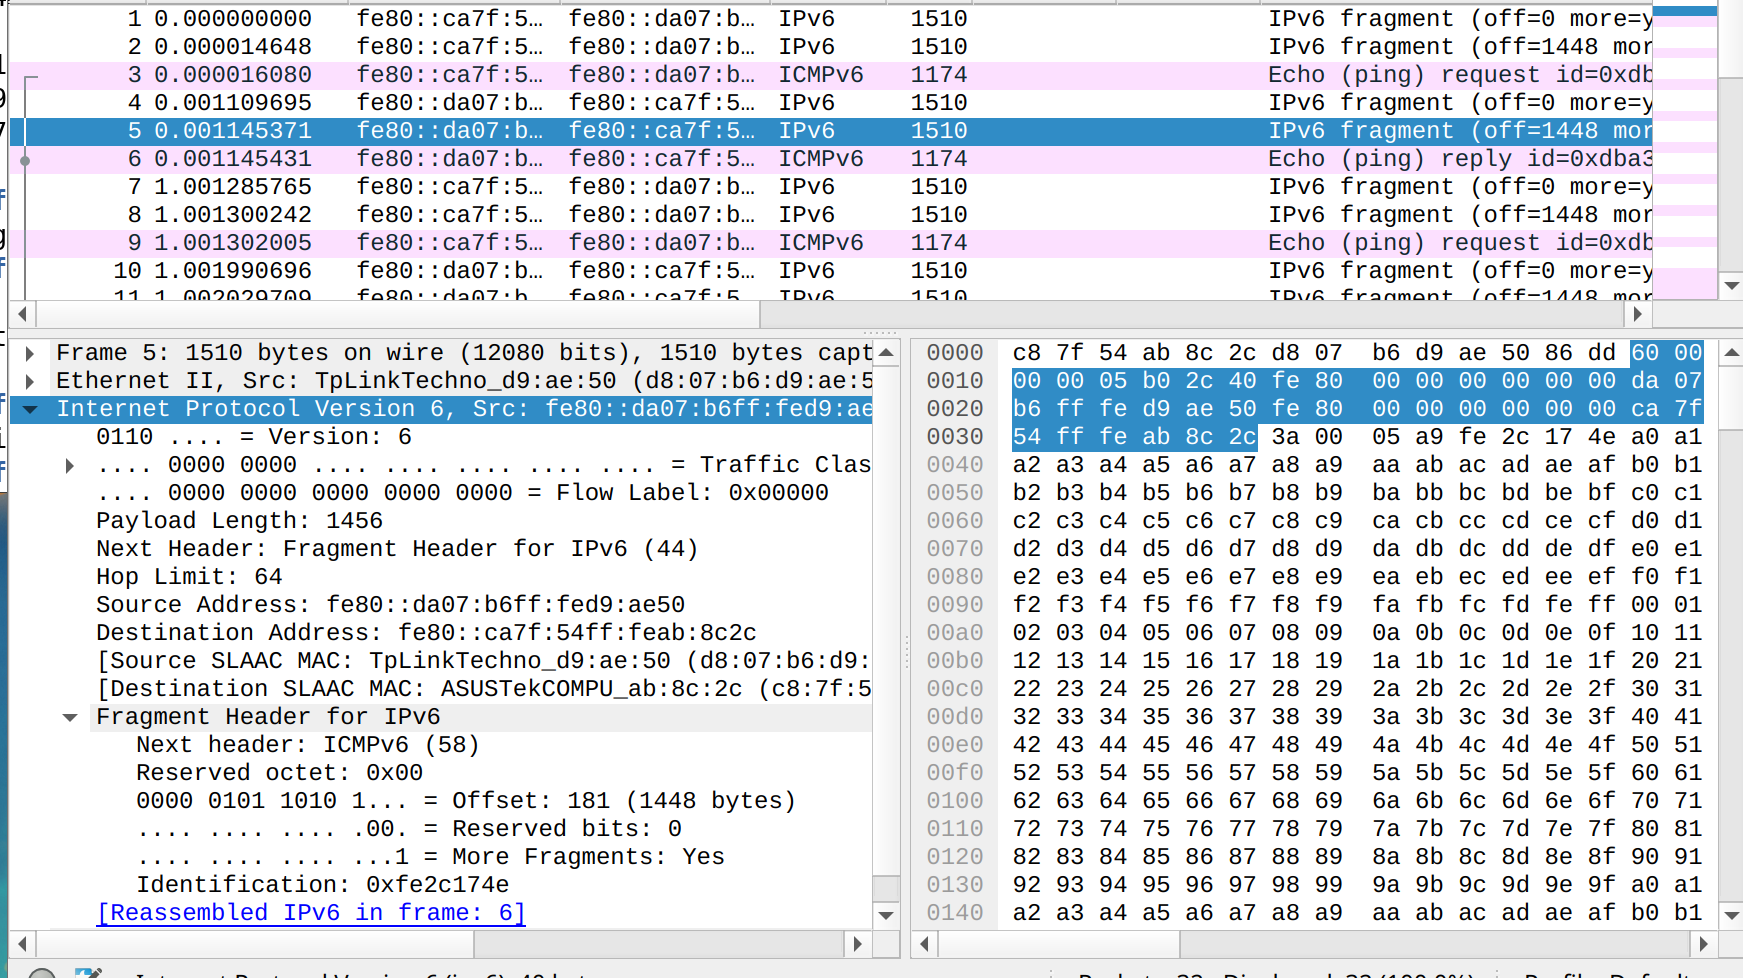
\includegraphics[width=\textwidth]{../routing/ipv6-fragment-ex}
\end{frame}

\begin{frame}{IPv4 fragments}
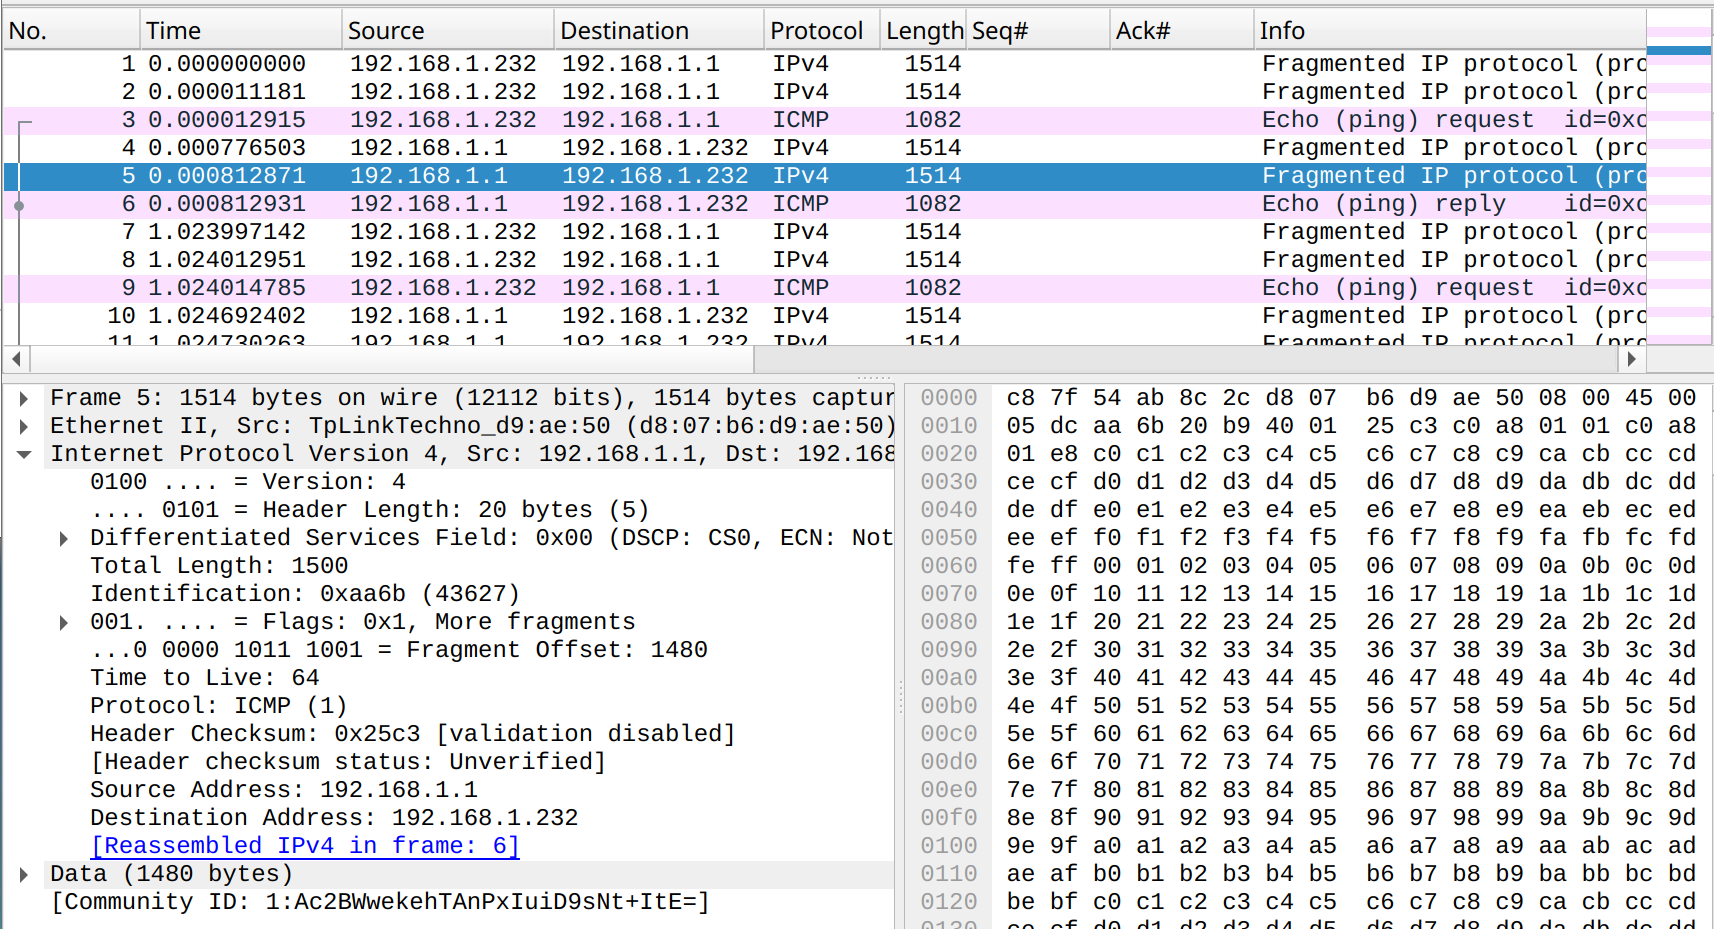
\includegraphics[width=\textwidth]{../routing/ipv4-fragment-ex}
\end{frame}

\begin{frame}{varying frame size support}
    \begin{itemize}
    \item also called \textit{maximum transmission unit} (MTU)
    \vspace{.5cm}
    \item typical Ethernet, Wifi --- 1500 bytes
    \item Ethernet with ``jumbo frames'' -- 65535 bytes
    \item IPsec ESP VPN over 1500-byte MTU network -- $\sim$1400--1440 bytes
        \begin{itemize}
        \item VPN --- simulated network link over other network links
        \end{itemize}
    \end{itemize}
\end{frame}

\begin{frame}{routers making fragments}
    \begin{itemize}
    \item option in IPv4 to handle frame size mismatch, but not great:
    \vspace{.5cm}
    \item extra data sent over network (especially if just over max size)
        \begin{itemize}
        \item extra copies of main headers on each fragment
        \end{itemize}
    \item extra work at receiver to reconstruct fragments
    \item lose whole packet if one fragment is lost
        \begin{itemize}
        \item but other routers likely to still waste time forwarding all other fragments
        \end{itemize}
    \end{itemize}
\end{frame}

\begin{frame}{avoiding fragmentation}
    \begin{itemize}
    \item IPv4 --- DF (don't fragment) flag in packets
        \begin{itemize}
        \item if set, routers not allowed to fragment packet
        \end{itemize}
    \item IPv6 --- routers never fragment packets
        \begin{itemize}
        \item any fragments made at source machine only
        \end{itemize}
    \vspace{.5cm}
    \item<2-> when set --- ICMP error
        \begin{itemize}
        \item ICMPv6: Packet Too Big
        \item ICMPv4: destination unreachable + reason code of fragmentation needed
        \item (hopefully, bad networks might drop packet instead)
        \end{itemize}
    \item<2-> ICMPv6 error tells you maximum supported size
        \begin{itemize}
        \item (by first link that got packet rejected --- might be more constraining link later)
        \item info not available in IPv4
        \end{itemize}
    \end{itemize}
\end{frame}
 % FIXME: IP packet format

% FIXME: exercise on fragmentation perf impact
\subsubsection{exercise}
\begin{frame}{exercise: fragmentation perf}
    \begin{itemize}
    \item assume:
    \begin{itemize}
        \item Ethernet header/trailer: 26 bytes
        \item IPv4 header: 20 bytes + 0 bytes of options
        \item TCP header: 20 bytes + 16 bytes of options
    \end{itemize}
    \vspace{.5cm}
    \item suppose local network supports 65535-byte ethernet payloads
    \item and remote network suports 1500-byte ethernet payloads
    \item and fragmentation happens
    \item exericses:
        \begin{itemize}
        \item lowest overhead TCP segment size?
        \item overhead for 64000-byte TCP segments?
        \item highest overhead TCP segment size?
        \end{itemize}
    \end{itemize}
\end{frame}


\subsection{time-to-live}

\againframe<4>{forwardProbs}
\begin{frame}{time-to-live (v4) / hop limit (v6)}
    \begin{itemize}
    \item stored in IP header 
    \vspace{.5cm}
    \item when forwarding packet, router will:
    \item subtract one from TTL / hop limit
        \begin{itemize}
        \item and recompute checksum accordingly
        \end{itemize}
    \item if TTL/hop limit = 0, drop packet
    \item usually send back ICMP ``Time Exceeded'' error
    \end{itemize}
\end{frame}



\section{traceroute}

\begin{frame}{traceroute}
    \begin{itemize}
    \item ICMP Time Exceeded messages come from router
    \item $\rightarrow$ tells you which routers are involved
    \vspace{.5cm}
    \item<2-> \texttt{traceroute} command: deliberately packets with low TTL/hop limit
    \item<2-> print out what time exceeded messages we get back
    \item<2-> typically sent with TTL/hop limit = 255 so it doesn't get lost
        \begin{itemize}
        \item (`backwards' path might be longer than forwards one)
        \end{itemize}
    \end{itemize}
\end{frame}

\begin{frame}[fragile]{traceroute example}
\begin{Verbatim}[fontsize=\fontsize{8}{9}\selectfont]
traceroute to ripe.net (193.0.11.51), 30 hops max, 60 byte packets
 1  128.143.63.1 (128.143.63.1)  6.367 ms  8.562 ms  8.577 ms
 2  cr01-gil-ae15-00.net.virginia.edu (128.143.221.17)  0.370 ms  0.334 ms  0.349 ms
 3  * * *
 4  br01-udc-et-1-2-0.net.virginia.edu (128.143.236.5)  0.502 ms  0.468 ms  0.488 ms
 5  i2-vt.net.virginia.edu (192.35.48.34)  3.374 ms  3.448 ms  3.413 ms
 6  192.122.175.15 (192.122.175.15)  5.715 ms  5.628 ms  5.590 ms
 7  fourhundredge-0-0-0-17.4079.core1.ashb.net.internet2.edu (163.253.1.8)  29.163 ms
    fourhundredge-0-0-0-16.4079.core1.ashb.net.internet2.edu (163.253.1.2)  28.880 ms
    fourhundredge-0-0-0-17.4079.core1.ashb.net.internet2.edu (163.253.1.8)  28.876 ms
 8  fourhundredge-0-0-0-1.4079.core1.clev.net.internet2.edu (163.253.1.123)  29.568 ms 
    28.667 ms  28.666 ms
 9  fourhundredge-0-0-0-0.4079.core2.newy32aoa.net.internet2.edu (163.253.1.239)  29.608 ms 
    29.476 ms  29.400 ms
10  fourhundredge-0-0-0-19.4079.core1.newy32aoa.net.internet2.edu (163.253.1.40)  28.958 ms 
    28.999 ms 
    fourhundredge-0-0-0-21.4079.core1.newy32aoa.net.internet2.edu (163.253.1.44)  29.280 ms
11  e1-3-2-502.asd001b-jnx-06.surf.net (145.145.166.18)  115.822 ms  115.823 ms  115.744 ms
12  lo0-2.asd001b-jnx-01-surfinternet.surf.net (145.145.128.4)  115.988 ms  115.932 ms  115.918 ms
13  gw.amsix.telrtr.ripe.net (80.249.208.71)  121.956 ms  121.968 ms  121.844 ms
14  * * *
15  * * *
\end{Verbatim}
\end{frame}

\begin{frame}{traceroute sent}
% FIXME: screenshot
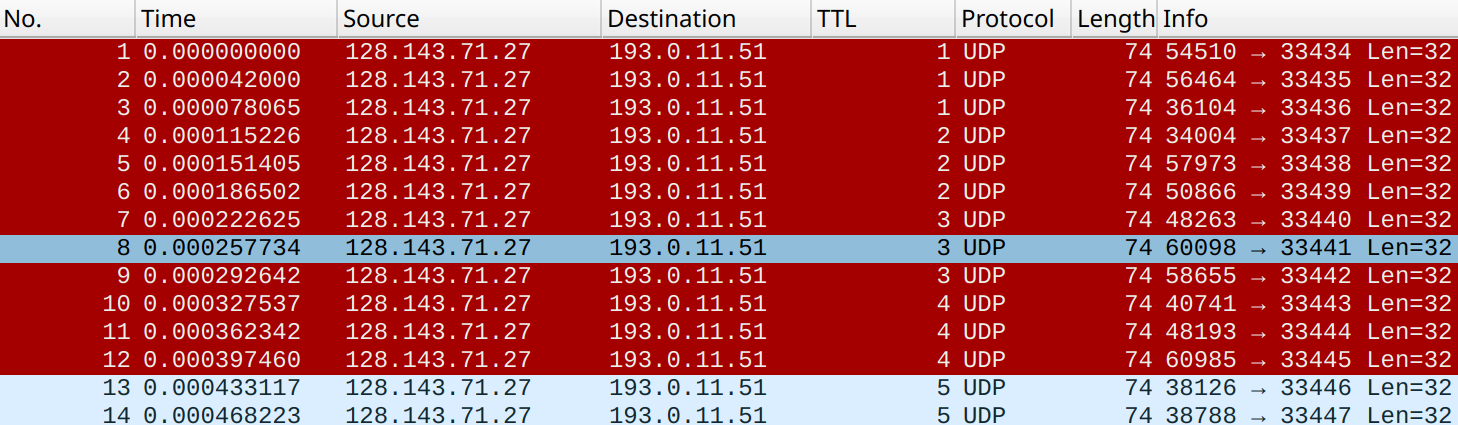
\includegraphics[width=\textwidth]{../routing/traceroute-v4-send}
\end{frame}

\begin{frame}{traceroute received}
% FIXME: screenshot
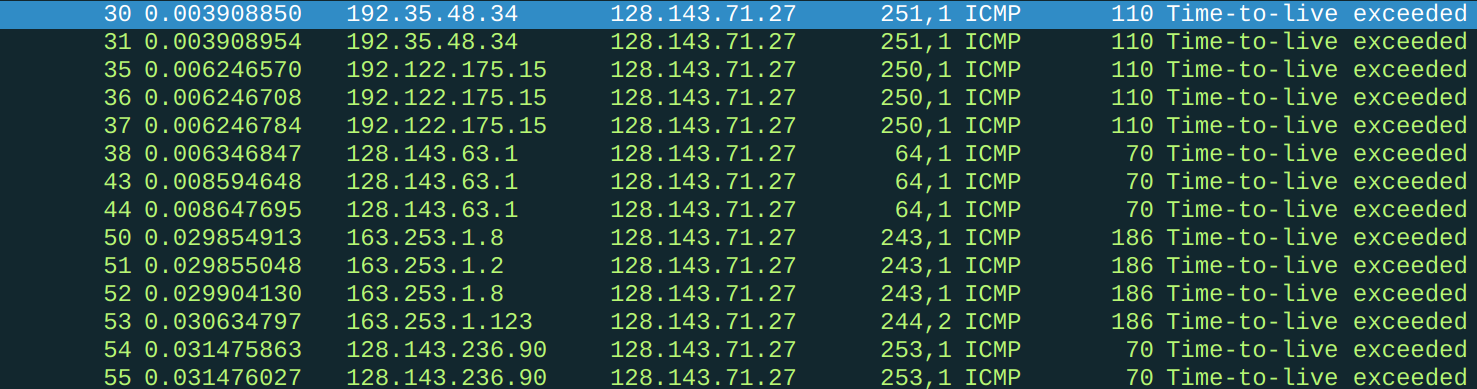
\includegraphics[width=\textwidth]{../routing/traceroute-v4-recv}
\end{frame}

\begin{frame}{aside: multiple paths}
    \begin{itemize}
    \item only showing \textit{forward} path
        \begin{itemize}
        \item routing in reverse direction is often different
        \end{itemize}
    \item sometimes multiple forward paths
        \begin{itemize}
        \item way we've shown routing table so far does not allow this
        \end{itemize}
    \end{itemize}
\end{frame}


\section{centralized versus distributed}
\begin{frame}{constructing routing/neighbor tables}
    \begin{itemize}
    \item interesting task: how to fill tables
    \item two general strategies:
    \vspace{.5cm}
    \item routers/switches learn from neighbors
        \begin{itemize}
        \item ``distributed''
        \end{itemize}
    \item information gathered on single controller machine \\
        which configures routers/switches
        \begin{itemize}
        \item ``centralized''
        \end{itemize}
    \end{itemize}
\end{frame}


\section{basic flooding / MAC learning}
% FIXME
\usetikzlibrary{arrows.meta,calc,matrix,shapes}
\providecommand{\computer}{%
    
\includegraphics[width=1cm]{../common/Noun_project_216.pdf}
}
\providecommand{\switch}{%
    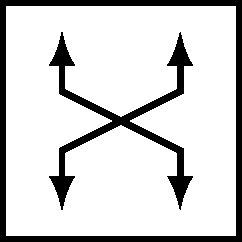
\includegraphics[width=0.9cm]{../common/fig-switch.pdf}
}
\providecommand{\router}{%
    
\includegraphics[width=0.9cm]{../common/fig-router.pdf}
}

\begin{frame}{basic flooding}
    \begin{itemize}
    \item idea: broadcast message to whole network
    \item where message comes from = way to send back
    \vspace{.5cm}
    \item used this idea in MAC learning
    \end{itemize}
\end{frame}

\begin{frame}{flooding one entry}
\begin{tikzpicture}
\tikzset{
    computer/.style={inner sep=0mm,outer sep=0mm,execute at begin node={\computer}},
    switch/.style={inner sep=0mm,outer sep=0mm,execute at begin node={\switch}},
    connect/.style={draw,very thick,Latex-Latex},
    connect big/.style={draw,ultra thick,Latex-Latex},
    port/.style={pos=0.95,fill=white,circle,draw,inner sep=0mm},
    port beginning/.style={pos=0.05,fill=white,circle,draw,inner sep=0mm},
    route table/.style={
        matrix of nodes,ampersand replacement=\&,
        column 1/.style={nodes={draw,thick,text width=2.5cm,font=\tiny\tt,text depth=0mm,minimum height=0.5cm,inner sep=1mm}},
        column 2/.style={nodes={draw,thick,text width=.5cm,font=\small\tt,text depth=0mm,minimum height=0.5cm,inner sep=1mm}},
        row 1/.style={nodes={draw=none,font=\small}},
    },
    mac label/.style={
        draw,fill=white,inner sep=1mm,font=\tiny\tt,
    },
}
\foreach \x/\d/\mc/\dir in {15/8cm/AA/north,45/3cm/BB/north,90/2cm/CC/north,135/3cm/DD/north,180/4cm/EE/north,300/4cm/FF/south} {
    \node[computer,label={[mac label,]\dir:00:11:22:33:44:\small\mc}] (c-\x) at (\x:\d) {};
}
\node[switch] (s1) at (4,-0.5) {};
\matrix[route table,anchor=north west,
    row 3/.style={nodes={visible on=<2->,alt=<2>{fill=red!10}}},
] (s1 table) at ([xshift=1cm,yshift=.5cm]s1.north east) {
dst MAC addr \& port \\
\ldots \& \ldots \\
00:11:22:33:44:\small AA \& 1 \\
};
\draw[dotted,thick] (s1.north east) -- (s1 table-2-1.north west);
\draw[dotted,thick] (s1.south east) -- (s1 table-2-1.south west);
\node[switch] (s2) at (-1,0.5) {};
\matrix[route table,
    row 3/.style={nodes={visible on=<3->}},
,anchor=north east] (s2 table) at ([xshift=3cm]s2.south west) {
dst MAC addr \& port \\
\ldots \& \ldots \\
00:11:22:33:44:\small AA \& 1 \\
};
\draw[dotted,thick] (s2.south east) -- (s2 table-2-2.north east);
\draw[dotted,thick] (s2.south west) -- (s2 table-2-1.north west);
\node[switch] (s3) at (-4,-3) {};
\matrix[route table,
    row 3/.style={nodes={visible on=<4->}},
,anchor=north west] (s3 table) at ([xshift=1cm,yshift=0.5cm]s3.north east) {
dst MAC addr \& port \\
\ldots \& \ldots \\
00:11:22:33:44:\small AA \& 2 \\
};
\draw[dotted,thick] (s3.south east) -- (s3 table-2-2.north east);
\draw[dotted,thick] (s3.south west) -- (s3 table-2-1.north west);
\draw[connect] (c-15) -- (s1) node[port] {1}
    node[midway,visible on=<2>,draw=red,fill=red!10] {from \ldots:AA};
\draw[connect] (c-45) -- (s1) node[port] {2};
\draw[connect] (c-300) -- (s1) node[port] {3};
\draw[connect] (c-90) -- (s2) node[port] {2};
\draw[connect] (c-135) -- (s2) node[port] {3};
\draw[connect] (c-180) -- (s2) node[port] {4};
\draw[connect big] (s1) -- (s2) node[port beginning] {4} node [port] {1}
    node[midway,visible on=<3>,draw=red,fill=red!10] {from \ldots:AA};
\draw[connect big] (s2) -- (s3) node[port beginning] {5} node [port] {2}
    node[midway,visible on=<4>,draw=red,fill=red!10] {from \ldots:AA};
\end{tikzpicture}
\end{frame}

\begin{frame}{`flooding'}
\begin{tikzpicture}
\tikzset{
    computer/.style={inner sep=0mm,outer sep=0mm,execute at begin node={\computer}},
    switch/.style={inner sep=0mm,outer sep=0mm,execute at begin node={\switch}},
    router/.style={inner sep=0mm,outer sep=0mm,execute at begin node={\router}},
    connect/.style={draw,very thick,Latex-Latex},
    connect big/.style={draw,ultra thick,Latex-Latex},
    port/.style={pos=0.95,fill=white,circle,draw,inner sep=0mm},
    port beginning/.style={pos=0.05,fill=white,circle,draw,inner sep=0mm},
    route table/.style={
        matrix of nodes,ampersand replacement=\&,
        column 1/.style={nodes={draw,thick,text width=2.2cm,font=\fontsize{7}{8}\selectfont\tt\strut,minimum height=0.4cm,inner sep=.2mm}},
        column 2/.style={nodes={draw,thick,text width=2.1cm,font=\fontsize{7}{8}\selectfont\tt\strut,minimum height=0.4cm,inner sep=.2mm}},
        column 3/.style={nodes={draw,thick,text width=.7cm,font=\fontsize{7}{8}\selectfont\tt\strut,minimum height=0.4cm,inner sep=.2mm}},
        row 1/.style={nodes={draw=none,font=\fontsize{9}{10}\selectfont}},
    },
    mac label/.style={
        draw,fill=white,inner sep=1mm,font=\tiny\tt,
    },
    s label/.style={
        font=\fontsize{8}{9}\tt\selectfont,align=center
    },
    net cloud/.style={cloud,draw,very thick,aspect=2},
    send out/.style={draw=violet,line width=1.5mm,dotted,-Latex},
    sent out info/.style={solid,draw=violet,line width=1mm,fill=white,align=left,font=\small\tt},
}
\node[router,label={[s label]north:(0) 2001:db8:1::1\\(1) 2001:db8:f::1},
    alt=<5>{fill=red!10},] (s1) at (3, 2) {};
\node[net cloud] (s1 cloud) at (1, 2.5) {};
\draw[connect] (s1) -- (s1 cloud) node[port beginning] {0};
\matrix[route table,anchor=north east] (s1 table) at ([xshift=-1cm]s1.north west) {
    addresses \& gateway \& port \\
    2001:db8:1::/40 \& --- \& 0 \\
    2001:db8:f::/40 \& --- \& 1 \\
};
\node[router,label={[s label]south:(0) 2001:db8:f::2\\(1) 2001:db8:2::1}] (s2) at (3, 0) {};
\draw[connect] (s1) -- (s2) node[port beginning] {1} node[port] {0};
\node[net cloud] (s2 cloud) at (6, 0) {};
\draw[connect] (s2) -- (s2 cloud) node[port beginning] {1};
\matrix[route table,anchor=north east,
    row 4/.style={nodes={visible on=<4->,alt=<4>{fill=red!10}}},
    row 5/.style={nodes={visible on=<5->,alt=<5>{fill=red!10}}},
] (s2 table) at ([xshift=-1cm]s2.north west) {
    addresses \& gateway \& port \\
    2001:db8:f::/40 \& --- \& 0 \\
    2001:db8:2::/40 \& --- \& 1 \\
    2001:db8:4::/40 \& 2001::db8:2::3 \& 1 \\
    2001:db8:1::/40 \& 2001::db8:f::1 \& 0 \\
};
\node[router,label={[s label]east:(0) 2001:db8:2::2\\(1) 2001:db8:3::1}] (s3) at (6, 1.5) {};
\draw[connect] (s2 cloud) -- (s3) node[port] {0};
\matrix[route table,anchor=south,
    row 4/.style={nodes={visible on=<4->,alt=<4>{fill=red!10}}},
    row 5/.style={nodes={visible on=<6->}},
    row 6/.style={nodes={visible on=<6->}},
    overlay,
    alt={<6>{row 5/.style={nodes={fill=red!10}}}},
    alt={<6>{row 6/.style={nodes={fill=red!10}}}},
] (s3 table) at ([xshift=1.5cm]s3.north) {
    addresses \& gateway \& port \\
    2001:db8:2::/40 \& --- \& 0 \\
    2001:db8:3::/40 \& --- \& 1 \\
    2001:db8:4::/40 \& 2001:db8:2::3\& 0 \\
    2001:db8:f::/40 \& 2001:db8:2::1\& 0 \\
    2001:db8:1::/40 \& 2001:db8:2::1\& 0 \\
};
\node[router,alt=<2-3>{fill=red!10},
      label={[s label]east:(0) 2001:db8:2::3\\(1) 2001:db8:4::1}] (s4) at (6, -1.5) {};
\draw[connect] (s2 cloud) -- (s4) node[port,alt=<2-3>{fill=red!10}] {0};
\matrix[
    route table,anchor=north,
    row 3/.style={nodes={visible on=<2->}},
    row 4/.style={nodes={visible on=<6->}},
    row 5/.style={nodes={visible on=<6->}},
    alt={<2-4>{row 3/.style={nodes={fill=red!10}}}},
    alt={<6>{row 4/.style={nodes={fill=red!10}}}},
    alt={<6>{row 5/.style={nodes={fill=red!10}}}},
] (s4 table) at (s4.south) {
    addresses \& gateway \& port \\
    2001:db8:2::/40 \& --- \& 0 \\
    2001:db8:4::/40 \& 2001:db8:2::3 \& 1 \\
    2001:db8:f::/40 \& 2001:db8:2::1 \& 0 \\
    2001:db8:1::/40 \& 2001:db8:2::1 \& 0 \\
};
    \begin{visibleenv}<2>
        \node[align=left,font=\small,fill=white,anchor=west,draw=red,ultra thick] at (s3.south west) {
            find out where \\
            we can forward packets \\
            not using port 0
        };
    \end{visibleenv}
    \begin{visibleenv}<3-4>
        \draw[send out] (s4.north) -- (s2 cloud.center) -- (s2);
        \draw[send out] (s4.north) -- (s2 cloud.center) -- (s3);
        \node[sent out info,anchor=north west] at ([xshift=.5cm]s3.south) {
            via 2001:db8:2::3 \\
            2001:db8:3::/40
        };
    \end{visibleenv}
    \begin{visibleenv}<5>
        \draw[send out] (s1.south) -- (s2.north)
            node[midway, left=1cm, sent out info] {
                via 2001:db8:f::1 \\
                2001:db8:1::/40
            };
    \end{visibleenv}
    \begin{visibleenv}<6>
        \draw[send out] (s2.east) -- (s2 cloud.center) -- (s3.south);
        \draw[send out] (s2.east) -- (s2 cloud.center) -- (s4.north);
        \node[anchor=west,sent out info] at (s2 cloud.east)
            {
                via 2001:db8:2::1 \\
                2001::db8:f::/40 \\
                2001::db8:1::/40 
            };
    \end{visibleenv}
\end{tikzpicture}
\end{frame}

\begin{frame}{eventual convergence}
    \begin{itemize}
    \item `flooding' algorithm:
    \item periodically send on each network:
        \begin{itemize}
        \item list of routes you have that don't double-back to same network
        \end{itemize}
    \item when receiving routes sent on network:
        \begin{itemize}
        \item add routing table entry for each route
        \end{itemize}
    \vspace{.5cm}
    \item<2-> not handled: \myemph{multiple paths}?
    \end{itemize}
\end{frame}

\begin{frame}{only one path?}
    \begin{itemize}
    \item only one path on network means:
    \vspace{.5cm}
    \item if a link fails, bad news
    \item network forms a tree
    \end{itemize}
\end{frame}

\begin{frame}{routing like this?}
    \begin{itemize}
    \item for IP routing, generally want to have multiple paths
    \item \ldots but this is basically how MAC learning works
    \vspace{.5cm}
    \item but it requires a network that is a tree
    \item what if we don't start with one?
    \end{itemize}
\end{frame}


\section{spanning trees}
\usetikzlibrary{arrows.meta,calc,matrix,shapes}
\providecommand{\computer}{%
    
\includegraphics[width=1cm]{../common/Noun_project_216.pdf}
}
\providecommand{\switch}{%
    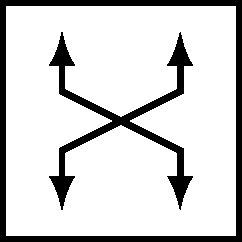
\includegraphics[width=0.9cm]{../common/fig-switch.pdf}
}
\providecommand{\router}{%
    
\includegraphics[width=0.9cm]{../common/fig-router.pdf}
}

\begin{frame}{spanning tree}
    \begin{itemize}
    \item given a general network, only activate subset of links
    \item \ldots such that network is tree
        \begin{itemize}
        \item that is only one path between each node
        \end{itemize}
    \vspace{.5cm}
    \item allows us to do flooding strategy
    \item makes simple MAC learning/broadcast just work
    \end{itemize}
\end{frame}

\begin{frame}{centralized spanning tree?}
    \begin{itemize}
    \item one algorithm you might learn in DSA2:
    \vspace{.5cm}
    \item mark one node called \textit{the root} as `in the tree'
    \item repeatedly: 
        \begin{itemize}
        \item add the `\myemph<2>{first}' link that goes to a node not in the tree
        \item mark newly connected node as `in the tree'
        \end{itemize}
    \vspace{.5cm}
    \item result = spanning tree
    \end{itemize}
\end{frame}

\begin{frame}{a careful ordering}
    \begin{itemize}
    \item algorithm works with any idea of which link/node is first
    \vspace{.5cm}
    \item we'll choose a particular ordering (for reasons you'll see later)
    \vspace{.5cm}
    \item first node one with earliest `name'
    \item links closer to the root before further links
    \item links from nodes with earlier names before later ones
    \end{itemize}
\end{frame}

\begin{frame}[fragile]{spanning tree example}
\begin{tikzpicture}
\tikzset{
    computer/.style={inner sep=0mm,outer sep=0mm,execute at begin node={\computer}},
    switch/.style={inner sep=0mm,outer sep=0mm,execute at begin node={\switch}},
    port/.style={pos=0.95,fill=white,circle,draw,inner sep=0mm},
    port beginning/.style={pos=0.05,fill=white,circle,draw,inner sep=0mm},
    route table/.style={
        matrix of nodes,ampersand replacement=\&,
        column 1/.style={nodes={draw,thick,text width=2.5cm,font=\tiny\tt,text depth=0mm,minimum height=0.5cm,inner sep=1mm}},
        column 2/.style={nodes={draw,thick,text width=.5cm,font=\small\tt,text depth=0mm,minimum height=0.5cm,inner sep=1mm}},
        row 1/.style={nodes={draw=none,font=\small}},
    },
    mac label/.style={
        draw,fill=white,inner sep=1mm,font=\tiny\tt,
    },
    tn/.style={draw,dotted,circle,very thick},
    real at/.style={alt=<#1->{solid},alt=<#1>{fill=red!10}},
    connect maybe/.style={draw,very thick,dotted,Latex-Latex},
    actual at/.style={alt=<#1->{draw=red,solid},alt=<#1>{draw,solid}},
    consider at/.style={alt=<#1>{draw=red}},
}
\node[tn,real at=1] (A) at (0, 0) {A};
\node[tn,real at=3] (B) at (5, -1) {B};
\node[tn,real at=4] (G) at (-5, -1) {G};
\node[tn,real at=6] (D) at (7, -3) {D};
\node[tn,real at=7] (E) at (1, -5) {E};
\node[tn,real at=8] (F) at (-7, -4) {F};
\draw[connect maybe,consider at=2,actual at=3] (A) -- (B)
    node[midway,sloped,above,visible on=<2>] {first priority};
\draw[connect maybe,consider at=2,actual at=4] (A) -- (G)
    node[midway,sloped,above,visible on=<2>] {second priority};
\draw[connect maybe,consider at=5] (B) -- (G)
    node[midway,sloped,below,visible on=<5>] {no new nodes};
\draw[connect maybe,actual at=6,consider at=5] (B) -- (D)
    node[midway,below left,visible on=<5>] {first priority};
\draw[connect maybe,actual at=8,consider at=5] (G) -- (F)
    node[midway,below right,visible on=<5>] {second priority};
\draw[connect maybe,consider at=6,actual at=7] (G) -- (E);
\draw[connect maybe,consider at=6] (D) -- (E);
\draw[connect maybe] (E) -- (F);
\end{tikzpicture}
\end{frame}

\begin{frame}{detecting `mistakes'}
    \begin{itemize}
    \item this method: consistent results every time
    \vspace{.5cm}
    \item but assumes we start from scratch
    \item we're going to want a way of doing this dynamically
    \vspace{.5cm}
    \item let's say we find a wrong configuration ---
    \item can we fix it?
    \end{itemize}
\end{frame}

\begin{frame}[fragile]{fixing wrong links}
\begin{tikzpicture}
\tikzset{
    computer/.style={inner sep=0mm,outer sep=0mm,execute at begin node={\computer}},
    switch/.style={inner sep=0mm,outer sep=0mm,execute at begin node={\switch}},
    port/.style={pos=0.95,fill=white,circle,draw,inner sep=0mm},
    port beginning/.style={pos=0.05,fill=white,circle,draw,inner sep=0mm},
    route table/.style={
        matrix of nodes,ampersand replacement=\&,
        column 1/.style={nodes={draw,thick,text width=2.5cm,font=\tiny\tt,text depth=0mm,minimum height=0.5cm,inner sep=1mm}},
        column 2/.style={nodes={draw,thick,text width=.5cm,font=\small\tt,text depth=0mm,minimum height=0.5cm,inner sep=1mm}},
        row 1/.style={nodes={draw=none,font=\small}},
    },
    mac label/.style={
        draw,fill=white,inner sep=1mm,font=\tiny\tt,
    },
    tn/.style={draw,dotted,circle,very thick},
    n real/.style={solid},
    n real at/.style={alt=<#1->{solid},alt=<#1>{fill=red!10}},
    n real until/.style={alt=<1-#1>{solid}},
    connect maybe/.style={draw,very thick,dotted,Latex-Latex},
    e real at/.style={alt=<#1>{draw=red,solid},alt=<#1->{draw,solid}},
    e real until/.style={alt=<1-#1>{solid},alt=<#1>{draw=red,solid}},
    e real/.style={solid},
    e hide up to/.style={alt=<1-#1>{invisible}},
    consider at/.style={alt=<#1>{draw=red,dotted}},
    explain box/.style={at={(0, -4)},align=center,draw=red,ultra thick,fill=white},
    explain box up/.style={at={(2, -1)},align=center,draw=red,ultra thick,fill=white},
}
\node[tn,n real] (A) at (0, 0) {A};
\node[tn,n real] (B) at (5, -1) {B};
\node[tn,n real] (G) at (-5, -1) {G};
\node[tn,n real] (D) at (7, -3) {D};
\node[tn,n real] (E) at (1, -5) {E};
\node[tn,n real] (F) at (-7, -4) {F};
\draw[connect maybe,e real] (A) -- (B);
\draw[connect maybe,e hide up to=1,e real at=2,consider at=2,alt=<3->{draw=black}] (A) -- (G);
\draw[connect maybe,e real until=2] (B) -- (G);
\draw[connect maybe,e real] (B) -- (D);
\draw[connect maybe,e real] (G) -- (F);
\draw[connect maybe,e hide up to=4,e real at=5] (G) -- (E);
\draw[connect maybe,e hide up to=2,alt=<3-4>{solid},alt=<3>{red},alt=<5>{red}] (D) -- (E);
\draw[connect maybe,e real until=3] (E) -- (F);
\begin{visibleenv}<2>
\node[explain box] {
    A--G beats B--G: closer to root
};
\end{visibleenv}
\begin{visibleenv}<3>
\node[explain box up] {
    D--F and F--E: \\
    same distance from root, but \\
    D before F, so D--E beats F--E
};
\end{visibleenv}
\begin{visibleenv}<5>
\node[explain box up] {
    G--E and D--E: \\
    G--E closer to root \\
    so G--E beats D--E
};
\end{visibleenv}
\end{tikzpicture}
\end{frame}

\begin{frame}{spanning tree protocol}
    \begin{itemize}
    \item each node tracks:
        \begin{itemize}
        \item what it believes is root of tree
        \item its link toward root of tree
        \item its distance to root of tree
        \item which other nodes think it's closer to root of tree
        \end{itemize}
    \item periodically sends information to neighbors
    \item when receiving information, update:
        \begin{itemize}
        \item root to lower ID number (if possible)
        \item link to lower-distance link  (if possible)
        \item link to lower-ID, same-distance link (if possible)
        \item which other nodes think it is closer
        \end{itemize}
    \end{itemize}
\end{frame}

\begin{frame}[fragile]{some example updates}
\begin{tikzpicture}
\tikzset{
    computer/.style={inner sep=0mm,outer sep=0mm,execute at begin node={\computer}},
    switch/.style={inner sep=0mm,outer sep=0mm,execute at begin node={\switch}},
    port/.style={pos=0.95,fill=white,circle,draw,inner sep=0mm},
    port beginning/.style={pos=0.05,fill=white,circle,draw,inner sep=0mm},
    route table/.style={
        matrix of nodes,ampersand replacement=\&,
        column 1/.style={nodes={draw,thick,text width=2.5cm,font=\tiny\tt,text depth=0mm,minimum height=0.5cm,inner sep=1mm}},
        column 2/.style={nodes={draw,thick,text width=.5cm,font=\small\tt,text depth=0mm,minimum height=0.5cm,inner sep=1mm}},
        row 1/.style={nodes={draw=none,font=\small}},
    },
    mac label/.style={
        draw,fill=white,inner sep=1mm,font=\tiny\tt,
    },
    n real/.style={solid},
    n real at/.style={alt=<#1->{solid},alt=<#1>{fill=red!10}},
    n real until/.style={alt=<1-#1>{solid}},
    tn/.style={draw,dotted,circle,very thick},
    real at/.style={alt=<#1->{solid},alt=<#1>{fill=red!10}},
    connect maybe/.style={draw,very thick,dotted,Latex-Latex},
    actual at/.style={alt=<#1->{draw=red,solid},alt=<#1>{draw,solid}},
    consider at/.style={alt=<#1>{draw=red}},
    msg link/.style={draw,violet,line width=1.2mm,-Latex},
    msg data/.style={draw=violet,line width=1mm,fill=white,align=left},
}
\node[tn,n real] (A) at (0, 0) {A};
\node[tn,n real] (B) at (5, -1) {B};
\node[tn,n real] (G) at (-5, -1) {G};
\node[tn,n real] (D) at (7, -3) {D};
\node[tn,n real] (E) at (1, -5) {E};
\node[tn,n real] (F) at (-7, -4) {F};
\draw[connect maybe] (A) -- (B);
\draw[connect maybe] (A) -- (G);
\draw[connect maybe] (B) -- (G);
\draw[connect maybe] (B) -- (D);
\draw[connect maybe] (G) -- (F);
\draw[connect maybe] (G) -- (E);
\draw[connect maybe] (D) -- (E);
\draw[connect maybe] (E) -- (F);
\tikzset{
    every node/.style={font=\small},
}
\begin{visibleenv}<2>
    \draw[msg link] (E) -- (G);
    \draw[msg link] (E) -- (F);
    \draw[msg link] (E) -- (D);
    \node[draw,very thick,anchor=south west] at (G.north east) {
        r=G,d=0,no link
    };
    \node[draw,very thick,alt=<2>{msg data},anchor=north] at (E.south) {
        r=E,d=0,no link
    };
    \node[draw,very thick,anchor=north west] at (F.south east) {
        r=F,d=0,no link
    };
    \node[draw,very thick,anchor=north west] at (D.south west) {
        r=D,d=0,no link
    };
\end{visibleenv}
\begin{visibleenv}<3>
    \draw[msg link] (E) -- (G);
    \draw[msg link] (E) -- (F);
    \draw[msg link] (E) -- (D);
    \node[draw,very thick,draw=red,anchor=south west] at (G.north east) {
        r=E,d=1,G--E
    };
    \node[draw,very thick,anchor=north] at (E.south) {
        r=E,d=0,no link
    };
    \node[draw,very thick,draw=red,anchor=north west] at (F.south east) {
        r=E,d=0,F--E
    };
    \node[align=left,draw,very thick,draw=red,anchor=north east] at (D.south west) {
        r=D,d=0,no link \\
        (D < G, so no update)
    };
\end{visibleenv}
\begin{visibleenv}<4>
    \draw[msg link] (D) -- (B);
    \draw[msg link] (D) -- (E);
    \node[draw,very thick,anchor=south west] at (G.north east) {
        r=E,d=1,G--E
    };
    \node[draw,very thick,anchor=north] at (E.south) {
        r=E,d=0,no link
    };
    \node[draw,very thick,anchor=north west] at (F.south east) {
        r=E,d=0,F--E
    };
    \node[draw,very thick,alt=<4>{msg data},anchor=north east] at (D.south west) {
        r=D,d=0,no link
    };
    \node[draw,very thick,anchor=south] at (B.north) {
        r=B,d=0,no link
    };
\end{visibleenv}
\begin{visibleenv}<5>
    \draw[msg link] (D) -- (B);
    \draw[msg link] (D) -- (E);
    \node[draw,very thick,anchor=south west] at (G.north east) {
        r=E,d=1,G--E
    };
    \node[draw,very thick,draw=red,anchor=north] at (E.south) {
        r=D,d=1,E--D
    };
    \node[draw,very thick,anchor=north west] at (F.south east) {
        r=E,d=0,F--E
    };
    \node[draw,very thick,anchor=north east] at (D.south west) {
        r=D,d=0,no link
    };
    \node[align=left,draw,very thick,draw=red,anchor=south] at (B.north) {
        r=B,d=0,no link \\
        (B < D, no update)
    };
\end{visibleenv}
\end{tikzpicture}
\end{frame}

\begin{frame}{spanning trees in practice (1)}
    \begin{itemize}
    \item commonly used on Ethernet for switches
    \item links not in spanning tree are `blocked'
        \begin{itemize}
        \item not used for normal traffic
        \item assumption: would cause loop $\rightarrow$ infinite packets
        \end{itemize}
    \item delay before activating port
        \begin{itemize}
        \item avoid temporary routing loops while figuring out tree
        \end{itemize}
    \item periodically send updates to all neighbors
        \begin{itemize}
        \item order of seconds
        \end{itemize}
    \end{itemize}
\end{frame}

\begin{frame}{spanning tree in practice (2)}
    \begin{itemize}
    \item real protocol supports variable `cost' for links
        \begin{itemize}
        \item so `distance to root' might be lower for faster links
        \end{itemize}
    \item modern variant (Rapid Spanning Tree Protocol) selects ``backup'' port to root 
        \begin{itemize}
        \item goal: faster switchover on failure
        \end{itemize}
    \end{itemize}
\end{frame}


\section{preview: better routing}
\begin{frame}[fragile]{exercise: best routes?}
\begin{tikzpicture}
\tikzset{
    computer/.style={inner sep=0mm,outer sep=0mm,execute at begin node={\computer}},
    switch/.style={inner sep=0mm,outer sep=0mm,execute at begin node={\switch}},
    port/.style={pos=0.95,fill=white,circle,draw,inner sep=0mm},
    port beginning/.style={pos=0.05,fill=white,circle,draw,inner sep=0mm},
    route table/.style={
        matrix of nodes,ampersand replacement=\&,
        column 1/.style={nodes={draw,thick,text width=2.5cm,font=\tiny\tt,text depth=0mm,minimum height=0.5cm,inner sep=1mm}},
        column 2/.style={nodes={draw,thick,text width=.5cm,font=\small\tt,text depth=0mm,minimum height=0.5cm,inner sep=1mm}},
        row 1/.style={nodes={draw=none,font=\small}},
    },
    mac label/.style={
        draw,fill=white,inner sep=1mm,font=\tiny\tt,
    },
    n real/.style={solid},
    n real at/.style={alt=<#1->{solid},alt=<#1>{fill=red!10}},
    n real until/.style={alt=<1-#1>{solid}},
    tn/.style={draw,dotted,circle,very thick},
    real at/.style={alt=<#1->{solid},alt=<#1>{fill=red!10}},
    connect maybe/.style={draw,very thick,dotted,Latex-Latex},
    actual at/.style={alt=<#1->{draw=red,solid},alt=<#1>{draw,solid}},
    consider at/.style={alt=<#1>{draw=red}},
    msg link/.style={draw,violet,line width=1.2mm,-Latex},
    msg data/.style={draw=violet,line width=1mm,fill=white,align=left},
}
\node[tn,n real] (A) at (0, 0) {A};
\node[tn,n real] (B) at (5, -1) {B};
\node[tn,n real] (G) at (-5, -1) {G};
\node[tn,n real] (D) at (7, -3) {D};
\node[tn,n real] (E) at (1, -5) {E};
\node[tn,n real] (F) at (-7, -4) {F};
\draw[connect maybe] (A) -- (B) node[midway,sloped,above] {1Mbit, 10ms};
\draw[connect maybe] (A) -- (G) node[midway,sloped,above] {10Mbit, 20ms};
\draw[connect maybe] (B) -- (G) node[midway,sloped,above] {11Mbit, 20ms};
\draw[connect maybe] (B) -- (D) node[midway,sloped,above] {5Mbit, 100ms};
\draw[connect maybe] (G) -- (F) node[midway,sloped,above] {6Mbit, 5ms};
\draw[connect maybe] (G) -- (E) node[midway,sloped,above] {8Mbit, 10ms};
\draw[connect maybe] (D) -- (E) node[midway,sloped,above] {2Mbit, 20ms};
\draw[connect maybe] (E) -- (F) node[midway,sloped,above] {100Mbit, 10ms};
\end{tikzpicture}
\begin{itemize}
\item A to B? B to E? F to G?
\end{itemize}
\end{frame}


\section{aside: metrics}
\begin{frame}{routing metrics}
    \begin{itemize}
    \item want some way of saying how `good' link is
    \item typically ``cost''/``distance'' value (so lower is better)
    \item in practice, most commonly \[\frac{\text{constant}}{\text{bandwidth}}\]
    \vspace{.5cm}
    \item could also try to:
        \begin{itemize}
        \item take financial costs into account
        \item take lantency into account
        \item take reliability into account
        \item spread flows out among more links
        \end{itemize}
    \end{itemize}
\end{frame}


\section{Bellman-Ford}
\usetikzlibrary{arrows.meta,matrix}
\begin{frame}{all-pairs Bellman-Ford}
    \begin{itemize}
    \item one algorithm to find all shortest paths in graph (network)
    \vspace{.5cm}
    \item $d(A,B) = \text{best distance from A to B}$
    \item $p(A,B) = \text{next node on path from A to B}$
    \item initially $d(X,X) = \infty$ for all nodes $X$
    \item repeatedly* do the following:
    \vspace{.5cm}
    \item for each link from A to B, distance $c$:
        \begin{itemize}
        \item for each node X:
        \item if $c + d(B, X) < d(A, X)$, \\
        \item then $d(A,X) \leftarrow c+d(B,X)$, $p(A,X) = B$
        \end{itemize}
    \end{itemize}
\end{frame}

\providecommand{\noroute}{$\infty$/---}
\providecommand{\mymark}[2]{\alt<#1->{\myemph<#1>{#2}}{}}
\begin{frame}[fragile]{running Bellman-Ford}
\begin{tikzpicture}
\tikzset{
    computer/.style={inner sep=0mm,outer sep=0mm,execute at begin node={\computer}},
    switch/.style={inner sep=0mm,outer sep=0mm,execute at begin node={\switch}},
    port/.style={pos=0.95,fill=white,circle,draw,inner sep=0mm},
    port beginning/.style={pos=0.05,fill=white,circle,draw,inner sep=0mm},
    route table/.style={
        matrix of nodes,ampersand replacement=\&,
        column 1/.style={nodes={draw,thick,text width=2.5cm,font=\tiny\tt,text depth=0mm,minimum height=0.5cm,inner sep=1mm}},
        column 2/.style={nodes={draw,thick,text width=.5cm,font=\small\tt,text depth=0mm,minimum height=0.5cm,inner sep=1mm}},
        row 1/.style={nodes={draw=none,font=\small}},
    },
    mac label/.style={
        draw,fill=white,inner sep=1mm,font=\tiny\tt,
    },
    n real/.style={solid},
    n real at/.style={alt=<#1->{solid},alt=<#1>{fill=red!10}},
    n real until/.style={alt=<1-#1>{solid}},
    tn/.style={draw,dotted,circle,very thick},
    real at/.style={alt=<#1->{solid},alt=<#1>{fill=red!10}},
    connect/.style={draw,very thick,-Latex},
    connect big/.style={draw,ultra thick,-Latex},
    actual at/.style={alt=<#1->{draw=red,solid},alt=<#1>{draw,solid}},
    consider at/.style={alt=<#1>{draw=red}},
    msg link/.style={draw,violet,line width=1.2mm,-Latex},
    msg data/.style={draw=violet,line width=1mm,fill=white,align=left},
}
\begin{scope}[x=0.8cm]
\node[tn,n real] (A) at (0, 0) {A};
\node[tn,n real] (B) at (5, -2) {B};
\node[tn,n real] (C) at (-5, -2) {C};
\node[tn,n real] (D) at (0, -4) {D};
\draw[connect big,alt=<2>{red}] ([yshift=1mm]A.east) -- ([xshift=1mm]B.north) node[midway,above] {2};
\draw[connect,alt=<3>{red},alt=<8>{red}] ([xshift=-1mm]B.north) -- ([yshift=-1mm]A.east) node[midway,below] {4};
\draw[connect big,alt=<7>{red}] ([yshift=1mm]A.west) -- ([xshift=-1mm]C.north) node[midway,above] {1};
\draw[connect big] ([xshift=1mm]C.north) -- ([yshift=-1mm]A.west) node[midway,below] {2};
\draw[connect big,alt=<5>{red}] ([yshift=1mm]C.east) -- ([yshift=1mm]B.west) node[midway,above] {2};
\draw[connect big,alt=<4>{red}] ([yshift=-1mm]B.west) -- ([yshift=-1mm]C.east) node[midway,below] {2};
\draw[connect,alt=<6>{red}] ([xshift=1mm]C.south) -- ([yshift=1mm]D.west) node[midway,above] {4};
\draw[connect] ([yshift=-1mm]D.west) -- ([xshift=-1mm]C.south) node[midway,below] {5};
\draw[connect big] ([xshift=-1mm]B.south) -- ([yshift=1mm]D.east) node[midway,above] {1};
\draw[connect big] ([yshift=-1mm]D.east) -- ([xshift=1mm]B.south) node[midway,below] {2};
\begin{visibleenv}<1-9>
\matrix[anchor=north west,tight matrix,
    nodes={font=\fontsize{10}{11}\selectfont,text width=1cm,minimum height=0.5cm}
] at (6, 0) {
    ~ \& A \& B \& C \& D \\
    A \& |[alt=<3>{fill=red!10}]| 0/A \& \only<1>{\noroute}\mymark{2}{2/B} \& \only<1-6>{\noroute}\mymark{7}{1/C} \& \only<1-6>{\noroute}\mymark{7}{5/D} \\
    B \& |[alt=<5>{fill=red!10}]| \only<1-2>{\noroute}\mymark{3}{4/A} \& |[alt=<2>{fill=red!10},alt=<5>{fill=red!10}]| 0/B\& \only<1-3>{\noroute}\mymark{4}{2/C} \& \only<1-7>{\noroute}{\mymark{8}{9/A}} \\
    C \& \only<1-4>{\noroute}\only<5->{\mymark{5}{6/B}} \& \only<1-4>{\noroute}\mymark{5}{2/B} \& 0/C \& 
            \only<1-5>{\noroute}{\mymark{6}{4/D}} \\
    D \& \noroute \& \noroute \& \noroute \& 0/D \\
};
\end{visibleenv}
\begin{visibleenv}<10>
\matrix[anchor=north west,tight matrix,
    nodes={font=\fontsize{10}{11}\selectfont,text width=1cm,minimum height=0.5cm}
] at (6, 0) {
    ~ \& A \& B \& C \& D \\
    A \& 0/A \& 2/B \& 4/C \& 3/B \\
    B \& 4/A \& 0/B \& 2/C \& 1/D \\
    C \& 2/A \& 2/B \& 0/C \& 4/D \\
    D \& 6/B \& 2/B \& 4/B \& 0/D \\
};
\end{visibleenv}
\end{scope}
\end{tikzpicture}
\end{frame}


\section{distance vector routing}
\subsection{distributing Bellman-Ford}
\usetikzlibrary{arrows.meta,matrix}

\providecommand{\noroute}{$\infty$/---}
\providecommand{\mymark}[2]{\alt<#1->{\myemph<#1>{#2}}{}}
\begin{frame}[fragile]{distributing Bellman-Ford}
\begin{tikzpicture}
\tikzset{
    computer/.style={inner sep=0mm,outer sep=0mm,execute at begin node={\computer}},
    switch/.style={inner sep=0mm,outer sep=0mm,execute at begin node={\switch}},
    port/.style={pos=0.95,fill=white,circle,draw,inner sep=0mm},
    port beginning/.style={pos=0.05,fill=white,circle,draw,inner sep=0mm},
    route table/.style={
        matrix of nodes,ampersand replacement=\&,
        column 1/.style={nodes={draw,thick,text width=2.5cm,font=\tiny\tt,text depth=0mm,minimum height=0.5cm,inner sep=1mm}},
        column 2/.style={nodes={draw,thick,text width=.5cm,font=\small\tt,text depth=0mm,minimum height=0.5cm,inner sep=1mm}},
        row 1/.style={nodes={draw=none,font=\small}},
    },
    mac label/.style={
        draw,fill=white,inner sep=1mm,font=\tiny\tt,
    },
    n real/.style={solid},
    n real at/.style={alt=<#1->{solid},alt=<#1>{fill=red!10}},
    n real until/.style={alt=<1-#1>{solid}},
    tn/.style={draw,dotted,circle,very thick},
    real at/.style={alt=<#1->{solid},alt=<#1>{fill=red!10}},
    connect/.style={draw,very thick,-Latex},
    connect big/.style={draw,ultra thick,-Latex},
    actual at/.style={alt=<#1->{draw=red,solid},alt=<#1>{draw,solid}},
    consider at/.style={alt=<#1>{draw=red}},
    msg link/.style={draw,violet,line width=1.2mm,-Latex},
    msg data/.style={draw=violet,line width=1mm,fill=white,align=left},
}
\begin{scope}[x=0.8cm]
\node[tn,n real] (A) at (0, 0) {A};
\node[tn,n real] (B) at (5, -2) {B};
\node[tn,n real] (C) at (-5, -2) {C};
\node[tn,n real] (D) at (0, -4) {D};
\draw[connect big] ([yshift=1mm]A.east) -- ([xshift=1mm]B.north) node[midway,above] {2};
\draw[connect] ([xshift=-1mm]B.north) -- ([yshift=-1mm]A.east) node[midway,below] {4};
\draw[connect big] ([yshift=1mm]A.west) -- ([xshift=-1mm]C.north) node[midway,above] {1};
\draw[connect big] ([xshift=1mm]C.north) -- ([yshift=-1mm]A.west) node[midway,below] {2};
\draw[connect big] ([yshift=1mm]C.east) -- ([yshift=1mm]B.west) node[midway,above] {2};
\draw[connect big] ([yshift=-1mm]B.west) -- ([yshift=-1mm]C.east) node[midway,below] {2};
\draw[connect] ([xshift=1mm]C.south) -- ([yshift=1mm]D.west) node[midway,above] {4};
\draw[connect] ([yshift=-1mm]D.west) -- ([xshift=-1mm]C.south) node[midway,below] {5};
\draw[connect big] ([xshift=-1mm]B.south) -- ([yshift=1mm]D.east) node[midway,above] {1};
\draw[connect big] ([yshift=-1mm]D.east) -- ([xshift=1mm]B.south) node[midway,below] {2};
\matrix[anchor=north west,tight matrix,
    nodes={font=\fontsize{10}{11}\selectfont,text width=1cm,minimum height=0.5cm},
    alt=<2>{
        row 2/.style={nodes={fill=violet!10}},
    },
    alt=<2>{
        row 3/.style={nodes={fill=green!10}},
    },
    alt=<2>{
        row 4/.style={nodes={fill=blue!10}},
    },
    alt=<2>{
        row 5/.style={nodes={fill=yellow!10}},
    },
    overlay,
] at (4, 2) {
    ~ \& A \& B \& C \& D \\
    A \& 0/A \& 2/B \& 1/C \& 5/D \\
    B \& 4/A \& 0/B\& 2/C \& 6/C \\
    C \& 1/A \& 2/B \& 0/C \& 4/D \\
    D \& \noroute \& \noroute \& \noroute \& 0/D \\
};
\begin{visibleenv}<2->
\tikzset{
    one dv/.style={
        tight matrix,
        nodes={alt=<2>{draw=red},fill=white,font=\fontsize{10}{11}\selectfont,text width=1cm,minimum height=0.5cm}
    }
}
\matrix[anchor=south,one dv,
    row 2/.style={nodes={fill=violet!10}},
] (A dv) at (A.north) {
    A \& B \& C \& D \\
    0/A \& 2/B \& 1/C \& 5/D \\
};
\matrix[anchor=north,one dv,
    row 2/.style={nodes={fill=yellow!10}},
] (D dv) at ([yshift=0cm]D.south) {
    A \& B \& C \& D \\
    \only<1-3>{\noroute}\mymark{4}{6/C} \& \only<1-6>{\noroute}\mymark{6}{7/B} \& \only<1-3>{\noroute}\mymark{4}{5/C} \& 0/D \\
};
\matrix[anchor=south west,one dv,
    row 2/.style={nodes={fill=blue!10}},
] (C dv) at ([xshift=-3cm]C.north east) {
    A \& B \& C \& D \\
    1/A \& 2/B \& 0/C \& 4/D \\
};
\matrix[anchor=north east,one dv,
    row 2/.style={nodes={fill=green!10}},
] (B dv) at ([yshift=.25cm,xshift=4cm]B.south west) {
    A \& B \& C \& D \\
     4/A \& 0/B\& 2/C \& 6/C \\
};
\end{visibleenv}
\begin{visibleenv}<1>
\node[fill=white,anchor=north,draw=red,ultra thick,align=center] at (1, 1) {
    store table row = ``distance vector'' on each node
};
\end{visibleenv}
\begin{visibleenv}<3-4>
\draw[msg link] (C) -- (D)
    node[midway,above,msg data] {I'm C, costs: A=1,B=2,C=0,D=5};
\end{visibleenv}
\begin{visibleenv}<3>
\node[fill=white,anchor=north,draw=red,ultra thick,align=center] at (1, 1) {
    nodes share their `distance vector' periodically\ldots
};
\end{visibleenv}
\begin{visibleenv}<4>
\node[fill=white,anchor=north,draw=red,ultra thick,align=center] at (1, 1) {
    when receiving distance vector \\
    see if new node (C) has better routes
};
\end{visibleenv}
\begin{visibleenv}<5>
\draw[msg link] (B) -- (D)
    node[midway,above,msg data] {I'm B, costs: A=4,B=0,C=2,D=5};
\node[fill=white,anchor=north,draw=red,ultra thick,align=center] at (1, 1) {
    exercise: what should change from update?
};
\end{visibleenv}
\end{scope}
\end{tikzpicture}
\end{frame}



\subsection{algorithm}
\begin{frame}{distance vector routing}
    \begin{itemize}
    \item each node keeps \textit{distance vector}
        \begin{itemize}
        \item distance to each other node (network)
        \item also which neighbor to go through to get that distance
        \end{itemize}
    \item periodically send distance vector to all neighbors
    \item when receiving distance vector from X, check
    \item ``would going through X give me a better distance?''
        \begin{itemize}
        \item if so, update distance + which neighbor
        \end{itemize}
    \end{itemize}
\end{frame}


\subsection{RIP}
\begin{frame}{Routing Information Protocol}
\begin{itemize}
\item router broadcast on networks it's connected to packet containing list of:
    \begin{itemize}
    \item networks it can reach (example: 1.2.3.0/24)
    \item its next hop to that network
    \item its metric (distance) to reach that network
    \end{itemize}
\item each router on that network processes that packet
\item on receiving distances, routers see if they can update their routes
    \begin{itemize}
    \item routes will be to networks (1.2.3.0/24, etc.), not routers
    \end{itemize}
\end{itemize}
\end{frame}

\begin{frame}{local information}
    \begin{itemize}
    \item routers need to track themselves:
    \vspace{.5cm}
    \item which networks they can reach directly
        \begin{itemize}
        \item (which networks is it connected to)
        \end{itemize}
    \item the `distance' it needs to reach those networks
        \begin{itemize}
        \item (probably based on its bandwidth to that network?)
        \end{itemize}
    \end{itemize}
\end{frame}

\begin{frame}{RIP --- when to update}
    \begin{itemize}
    \item policy: every approx. 30 seconds always AND
    \item immediately on changes (``triggered'')
    \vspace{.5cm}
    \item means that connecting new router should better routes quickly
    \end{itemize}
\end{frame}


\subsection{handling removal}
\usetikzlibrary{arrows.meta,matrix}

\providecommand{\noroute}{$\infty$/---}
\providecommand{\mymark}[2]{\alt<#1->{\myemph<#1>{#2}}{}}


\begin{frame}{links going down}
    \begin{itemize}
    \item problem with our update rule:
    \item assumes routes only get better
    \vspace{.5cm}
    \item reality: sometimes links go down
    \item need to find different route
    \end{itemize}
\end{frame}

\begin{frame}{updating for removal (1)}
    \begin{itemize}
    \item let's say I'm A and my distance vector is:
        \begin{itemize}
        \item A=0 via A, B=4 via B, C=5 via D, D=4 via D
        \end{itemize}
    \item if my link to D goes down, new distance vector should be?
        \begin{itemize}
        \item<2-> A=0 via A, B=4 via B, C=$\infty$ via no one, D=$\infty$ via no one
        \end{itemize}
    \vspace{.5cm}
    \item<2-> later updates might fix $\infty$s
    \end{itemize}
\end{frame}

\begin{frame}{updating for removal (2)}
    \begin{itemize}
    \item let's say I'm A and my distance vector is:
        \begin{itemize}
        \item B=4 via B, C=5 via D, D=4 via D
        \end{itemize}
    \item and D tells me its distance vector is
        \begin{itemize}
        \item B=8 via A, C=$\infty$ via no one, D=0 via D
        \end{itemize}
    \item then my (A)'s new distance vector should be?
        \begin{itemize}
        \item<2->B=4 via B, C=$\infty$ via no one, D=4 via D
        \end{itemize}
    \end{itemize}
\end{frame}

\begin{frame}{updating for removal (3)}
    \begin{itemize}
    \item let's say I'm A and my distance vector is:
        \begin{itemize}
        \item B=4 via B, C=5 via D, D=4 via D
        \end{itemize}
    \item and D tells me its distance vector is
        \begin{itemize}
        \item B=8 via A, C=5 via A, D=0 via D
        \end{itemize}
    \item then my (A)'s new distance vector should be?
        \begin{itemize}
        \item<2->B=4 via B, C=$\infty$ via no one, D=4 via D
        \end{itemize}
    \end{itemize}
\end{frame}

\begin{frame}{updating for removal (4)}
    \begin{itemize}
    \item let's say I'm A and my distance vector is:
        \begin{itemize}
        \item B=4 via B, C=5 via D, D=4 via D
        \end{itemize}
    \item and D tells me its distance vector is
        \begin{itemize}
        \item B=3 via B, C=8 via B, D=0 via D
        \end{itemize}
    \item then my (A)'s new distance vector should be?
        \begin{itemize}
        \item<2->B=4 via B, C=12 via D, D=4 via D
        \end{itemize}
    \vspace{.5cm}
    \item<2-> probably later update from B will overwrite route to C
    \end{itemize}
\end{frame}

\begin{frame}[fragile]{removal?}
\begin{tikzpicture}
\tikzset{
    computer/.style={inner sep=0mm,outer sep=0mm,execute at begin node={\computer}},
    switch/.style={inner sep=0mm,outer sep=0mm,execute at begin node={\switch}},
    port/.style={pos=0.95,fill=white,circle,draw,inner sep=0mm},
    port beginning/.style={pos=0.05,fill=white,circle,draw,inner sep=0mm},
    route table/.style={
        matrix of nodes,ampersand replacement=\&,
        column 1/.style={nodes={draw,thick,text width=2.5cm,font=\tiny\tt,text depth=0mm,minimum height=0.5cm,inner sep=1mm}},
        column 2/.style={nodes={draw,thick,text width=.5cm,font=\small\tt,text depth=0mm,minimum height=0.5cm,inner sep=1mm}},
        row 1/.style={nodes={draw=none,font=\small}},
    },
    mac label/.style={
        draw,fill=white,inner sep=1mm,font=\tiny\tt,
    },
    n real/.style={solid},
    n real at/.style={alt=<#1->{solid},alt=<#1>{fill=red!10}},
    n real until/.style={alt=<1-#1>{solid}},
    tn/.style={draw,dotted,circle,very thick},
    real at/.style={alt=<#1->{solid},alt=<#1>{fill=red!10}},
    connect/.style={draw,very thick,-Latex},
    connect big/.style={draw,ultra thick,-Latex},
    actual at/.style={alt=<#1->{draw=red,solid},alt=<#1>{draw,solid}},
    consider at/.style={alt=<#1>{draw=red}},
    msg link/.style={draw,violet,line width=1.2mm,-Latex},
    msg data/.style={draw=violet,line width=1mm,fill=white,align=left},
}
\begin{scope}[x=0.8cm]
\node[tn,n real] (A) at (0, 0) {A};
\node[tn,n real] (B) at (5, -2) {B};
\node[tn,n real] (C) at (-5, -2) {C};
\node[tn,n real] (D) at (0, -4) {D};
\draw[connect big] ([yshift=1mm]A.east) -- ([xshift=1mm]B.north) node[midway,above] {2};
\draw[connect] ([xshift=-1mm]B.north) -- ([yshift=-1mm]A.east) node[midway,below] {4};
\draw[connect big] ([yshift=1mm]A.west) -- ([xshift=-1mm]C.north) node[midway,above] {1};
\draw[connect big] ([xshift=1mm]C.north) -- ([yshift=-1mm]A.west) node[midway,below] {2};
\draw[connect big] ([yshift=1mm]C.east) -- ([yshift=1mm]B.west) node[midway,above] {2};
\draw[connect big] ([yshift=-1mm]B.west) -- ([yshift=-1mm]C.east) node[midway,below] {2};
\draw[connect] ([xshift=1mm]C.south) -- ([yshift=1mm]D.west) node[midway,above] {4};
\draw[connect] ([yshift=-1mm]D.west) -- ([xshift=-1mm]C.south) node[midway,below] {5};
\draw[connect big,alt=<1>{red},alt=<2>{dotted,black!20}] ([xshift=-1mm]B.south) -- ([yshift=1mm]D.east) node[midway,above] {1};
\draw[connect big,alt=<1>{red},alt=<2>{dotted,black!20}] ([yshift=-1mm]D.east) -- ([xshift=1mm]B.south) node[midway,below] {2};
\tikzset{
    one dv/.style={
        tight matrix,
        nodes={fill=white,font=\fontsize{10}{11}\selectfont,text width=1cm,minimum height=0.5cm}
    }
}
\matrix[anchor=south,one dv,
    row 2/.style={nodes={fill=violet!10}},
] (A dv) at (A.north) {
    A \& B \& C \& D \\
    0/A \& 2/B \& 4/C \& 3/B \\
};
\matrix[anchor=north,one dv,
    row 2/.style={nodes={fill=yellow!10}},
] (D dv) at ([yshift=0cm]D.south) {
    A \& B \& C \& D \\
    \only<1>{6/B}\mark{2}{\noroute} \& \only<1>{2/B}\mark{2}{\noroute} \& \only<1>{4/B}\mark{2}{\noroute} \& 0/D \\
};
\matrix[anchor=south west,one dv,
    row 2/.style={nodes={fill=blue!10}},
] (C dv) at ([xshift=-3cm]C.north east) {
    A \& B \& C \& D \\
    2/A \& 2/B \& 0/C \& 4/D \\
};
\matrix[anchor=north east,one dv,
    row 2/.style={nodes={fill=green!10}},
] (B dv) at ([yshift=.25cm,xshift=4cm]B.south west) {
    A \& B \& C \& D \\
    4/A \& 0/B \& 2/C \& \only<1>{1/D}\mark{2}{\noroute} \\
};
\end{scope}
\end{tikzpicture}
\end{frame}

 % FIXME: fill in diagram

\subsection{count-to-infinity}
\usetikzlibrary{arrows.meta,matrix}

\providecommand{\noroute}{$\infty$/---}
\providecommand{\mymark}[2]{\alt<#1->{\myemph<#1>{#2}}{}}


\begin{frame}[fragile]{count-to-infinity}
\begin{tikzpicture}
\tikzset{
    computer/.style={inner sep=0mm,outer sep=0mm,execute at begin node={\computer}},
    switch/.style={inner sep=0mm,outer sep=0mm,execute at begin node={\switch}},
    port/.style={pos=0.95,fill=white,circle,draw,inner sep=0mm},
    port beginning/.style={pos=0.05,fill=white,circle,draw,inner sep=0mm},
    route table/.style={
        matrix of nodes,ampersand replacement=\&,
        column 1/.style={nodes={draw,thick,text width=2.5cm,font=\tiny\tt,text depth=0mm,minimum height=0.5cm,inner sep=1mm}},
        column 2/.style={nodes={draw,thick,text width=.5cm,font=\small\tt,text depth=0mm,minimum height=0.5cm,inner sep=1mm}},
        row 1/.style={nodes={draw=none,font=\small}},
    },
    mac label/.style={
        draw,fill=white,inner sep=1mm,font=\tiny\tt,
    },
    n real/.style={solid},
    n real at/.style={alt=<#1->{solid},alt=<#1>{fill=red!10}},
    n real until/.style={alt=<1-#1>{solid}},
    tn/.style={draw,dotted,circle,very thick},
    real at/.style={alt=<#1->{solid},alt=<#1>{fill=red!10}},
    connect/.style={draw,very thick,-Latex},
    connect big/.style={draw,ultra thick,-Latex},
    actual at/.style={alt=<#1->{draw=red,solid},alt=<#1>{draw,solid}},
    consider at/.style={alt=<#1>{draw=red}},
    msg link/.style={draw,violet,line width=1.2mm,-Latex},
    msg data/.style={draw=violet,line width=1mm,fill=white,align=left},
}
\begin{scope}[x=0.8cm]
\node[tn,n real] (A) at (0, 0) {A};
\node[tn,n real] (B) at (5, -2) {B};
\node[tn,n real] (C) at (-5, -2) {C};
\node[tn,n real] (D) at (0, -4) {D};
\draw[connect big] ([yshift=1mm]A.east) -- ([xshift=1mm]B.north) node[midway,above] {2};
\draw[connect] ([xshift=-1mm]B.north) -- ([yshift=-1mm]A.east) node[midway,below] {4};
\draw[connect big] ([yshift=1mm]A.west) -- ([xshift=-1mm]C.north) node[midway,above] {1};
\draw[connect big] ([xshift=1mm]C.north) -- ([yshift=-1mm]A.west) node[midway,below] {2};
\draw[connect big] ([yshift=1mm]C.east) -- ([yshift=1mm]B.west) node[midway,above] {2};
\draw[connect big] ([yshift=-1mm]B.west) -- ([yshift=-1mm]C.east) node[midway,below] {2};
\draw[connect] ([xshift=1mm]C.south) -- ([yshift=1mm]D.west) node[midway,above] {4};
\draw[connect] ([yshift=-1mm]D.west) -- ([xshift=-1mm]C.south) node[midway,below] {5};
\draw[connect big,alt=<1>{red},alt=<2>{dotted,black!20}] ([xshift=-1mm]B.south) -- ([yshift=1mm]D.east) node[midway,above] {1};
\draw[connect big,alt=<1>{red},alt=<2>{dotted,black!20}] ([yshift=-1mm]D.east) -- ([xshift=1mm]B.south) node[midway,below] {2};
\tikzset{
    one dv/.style={
        tight matrix,
        nodes={fill=white,font=\fontsize{10}{11}\selectfont,text width=1cm,minimum height=0.5cm}
    }
}
\matrix[anchor=south,one dv,
    row 2/.style={nodes={fill=violet!10}},
] (A dv) at (A.north) {
    A \& B \& C \& D \\
    0/A \& 2/B \& 4/C \& \only<1-3>{3/B}\only<4->{\myemph<4>{8/B}} \\
};
\matrix[anchor=north,one dv,
    row 2/.style={nodes={fill=yellow!10}},
] (D dv) at ([yshift=0cm]D.south) {
    A \& B \& C \& D \\
    \noroute \& \noroute \& \noroute \& 0/D \\
};
\matrix[anchor=south west,one dv,
    row 2/.style={nodes={fill=blue!10}},
] (C dv) at ([xshift=-3cm]C.north east) {
    A \& B \& C \& D \\
    2/A \& 2/B \& 0/C \& \only<1>{\noroute}\only<2->{\myemph<2>{4/A}} \\
};
\matrix[anchor=north east,one dv,
    row 2/.style={nodes={fill=green!10}},
] (B dv) at ([yshift=.25cm,xshift=4cm]B.south west) {
    A \& B \& C \& D \\
    4/A \& 0/B \& 2/C \& \only<1-2>{\noroute}\only<3->{\myemph<3>{6/C}} \\
};
\begin{visibleenv}<2>
\draw[msg link] (A) -- (C);
\end{visibleenv}
\begin{visibleenv}<3>
\draw[msg link] (C) -- (B);
\end{visibleenv}
\begin{visibleenv}<4>
\draw[msg link] (B) -- (A);
\end{visibleenv}
\end{scope}
\end{tikzpicture}
\end{frame}

\begin{frame}{count-to-infinity}
    \begin{itemize}
    \item when node becomes unreachable, can have `phantom' routes
    \item keep propogating in loop, incrementing metric forever
    \vspace{.5cm}
    \item RIP solution: maximum metric is 15 (hops)
    \end{itemize}
\end{frame}

\begin{frame}{better count-to-infinity solutions?}
    \begin{itemize}
    \item can share information about more than just neighbors
    \vspace{.5cm}
    \item we'll see two examples:
    \item link-state routing protocols (example: OSPF)
        \begin{itemize}
        \item every router learns full map of network
        \end{itemize}
    \item border gateway protocol (BGP)
        \begin{itemize}
        \item (basically) track \textit{list of hops} alongside distances
        \item eliminate potential routes that would create duplicate hops (loops)
        \end{itemize}
    \end{itemize}
\end{frame}
 % FIXME: diagram

\section{link state}

\section{interdomain routing}

\subsection{business priorities}

\subsection{sharing routes: BGP}

\subsection{loop prevention, metrics}

\subsection{within-AS routing}

\subsection{hot or cold potato}

\section{backup slides}
\begin{frame}{backup slides}
\end{frame}

\end{document}
